\documentclass{article}%
\usepackage[T1]{fontenc}%
\usepackage[utf8]{inputenc}%
\usepackage{lmodern}%
\usepackage{textcomp}%
\usepackage{lastpage}%
\usepackage[head=40pt,margin=0.5in,bottom=0.6in]{geometry}%
\usepackage{graphicx}%
%
\title{\textbf{San Bernardino, belleza arquitectónica afectada por el exceso de basura}}%
\author{Sarahi Gómez Esaa | @SarahiEsaa}%
\date{17/10/2018}%
%
\begin{document}%
\normalsize%
\maketitle%
\textbf{URL: }%
http://www.el{-}nacional.com/noticias/sociedad/san{-}bernardino{-}belleza{-}arquitectonica{-}afectada{-}por{-}exceso{-}basura\_256043\newline%
%
\textbf{Periodico: }%
EN, %
ID: %
256043, %
Seccion: %
Sociedad\newline%
%
\textbf{Palabras Claves: }%
NO\_TIENE\newline%
%
\textbf{Derecho: }%
3.2, %
Otros Derechos: %
, %
Sub Derechos: %
3.2.1\newline%
%
\textbf{EP: }%
NO\newline%
\newline%
%
\textbf{\textit{En las esquinas de los colegios de la zona se acumulan los desechos de la comunidad. Los estudiantes deben soportar malos olores, moscas e incluso deben caminar sobre los desperdicios~}}%
\newline%
\newline%
%
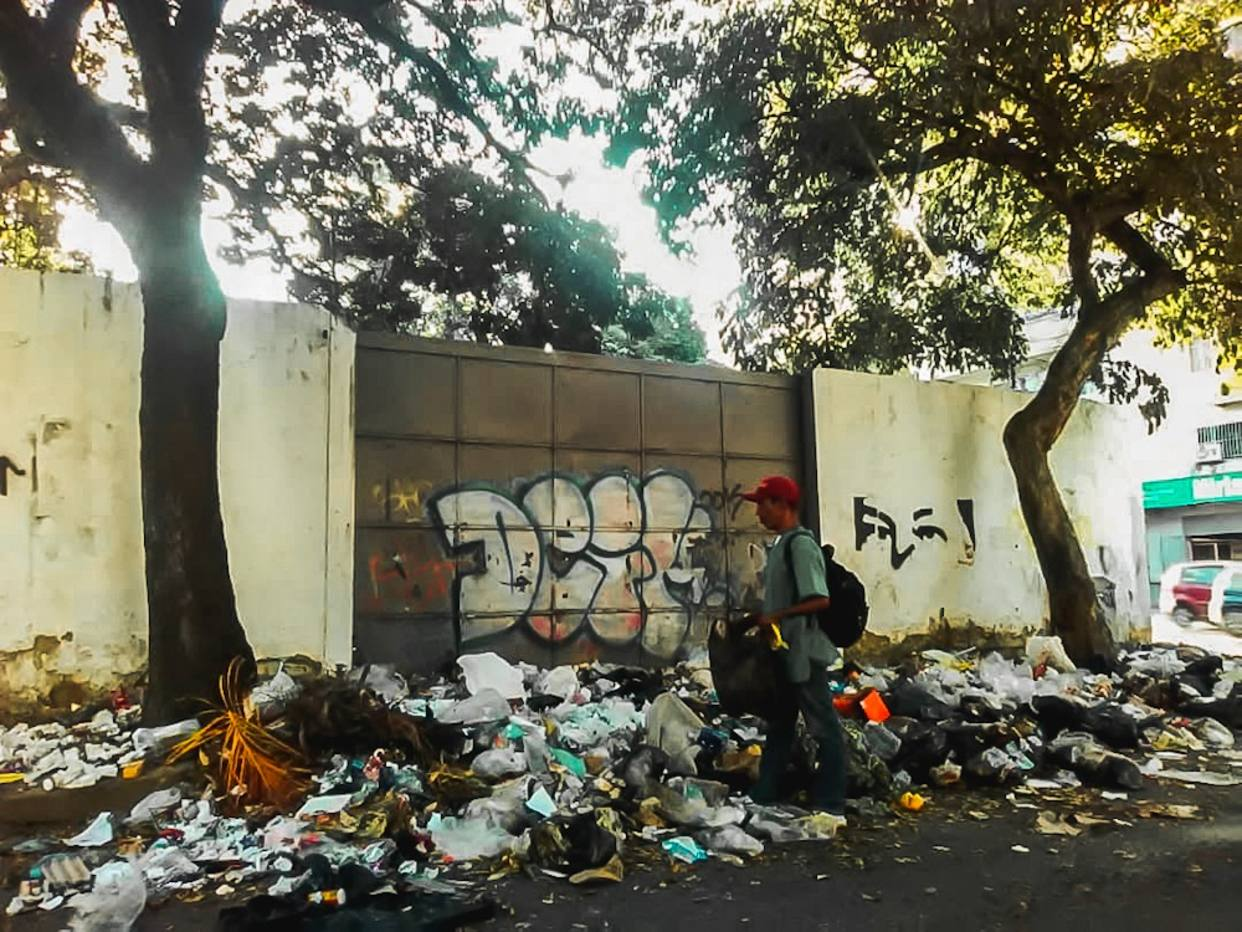
\includegraphics[width=300px]{186.jpg}%
\newline%
%
Las moscas y podredumbre se convirtieron en el compañero constante de los habitantes de San Bernardino, municipio Libertador de Caracas. Colegios y centros de salud se ven afectados por el crecimiento constante de los vertederos improvisados de basura.%
\newline%
%
La basura acumulada en las esquinas de la comunidad opaca la belleza arquitectónica de esta zona, que inició como una hacienda cafetalera y que dio paso a la construcción residencial en Caracas.%
\newline%
%
San Bernardino posee una gran cantidad de colegios y preescolares; sin embargo, la calidad educativa ha disminuido en cada uno de ellos por el crecimiento constante de los botaderos de basura.%
\newline%
%
Un vertedero de desechos de varios metros de longitud ubicado en la avenida Márquez del Toro afecta la salud y calidad de vida de dos unidades educativas, una de ellas es un preescolar, y dos centros de salud.%
\newline%
%
Vertedero improvisado ubicado en la avenida Marquéz del Toro. En frente se encuentra un colegio de educación inicial,~a media cuadra un liceo~~y dos centros de salud |~ Foto: Sarahi~Gómez%
\newline%
%
Este botadero se encuentra justo frente de una escuela de educación inicial. Jesús Rodríguez, director del preescolar, señaló a~El Nacional Web~~que la situación con la basura es complicada. Resaltó que la podredumbre y las moscas se meten a los salones de clases lo que hace muy difícil para los profesores impartir sus asignaturas.%
\newline%
%
“Mientras los niños comen necesitamos seis o siete personas que espanten las moscas”, dijo Rodríguez.%
\newline%
%
Denunció que cada vez que llaman a la alcaldía de Caracas para que recoja la basura les colocan excusas. “Nos dicen que no tienen vehículos o que no tienen personal”, dijo. ~La acumulación de desechos en esta zona lleva más de un mes lo que ha convertido el tránsito de niños y demás personas en una situación “insalubre”, según lo dicho por el director.%
\newline%
%
El vertedero cubre las raíces de los emblemáticos árboles de esta zona. Mientras un hombre revisa lo que puede comer o vender de los desechos, la podredumbre penetra el olfato agresivamente.%
\newline%
%
Vertedero de basura ubicado en la avenida Altamira. Justo al lado se encuentra un colegio. | Foto: Sarahí Gómez%
\newline%
%
En la avenida Altamira, la esquina de uno de los principales colegios de la zona se encuentra colapsada por los desechos. Los estudiantes deben bordear el vertedero de basura, plagado de moscas y gusanos, ~para llegar a la entrada del colegio.%
\newline%
%
Además de las plagas, el olor y el foco de infecciones ponen en riesgo la salud de los estudiantes y los residentes de la zona.%
\newline%
%
El exceso de basura no solo genera insalubridad sino que atrae a las personas en estado de indigencia. Un señor de aproximadamente 50 años~ de edad merodea los desperdicios, observa “por encima” lo que pueda utilizar de allí y se retira. Esta acción la repiten los demás indigentes de la zona quienes~ rompen las bolsas y los desperdicios se esparcen por la calle.%
\newline%
%
A una cuadra, otro botadero se observa en una esquina. Al lado, un liceo se enfrenta todos los días a los malos olores mientras que en frente la emergencia de una clínica atiende diariamente a pacientes.%
\newline%
%
Botadero de basura ubicado en la avenida Panteón, al lado se encuentra un liceo y en diagonal un centro de salud | Foto: Sarahi Gómez%
\newline%
%
Rodríguez exhortó a las autoridades a que se aboquen a la recolección de basura de la zona, sobre todo por la salud de los estudiantes.%
\newline%
%
En la plaza La Estrella, a menos de 20 metros de un colegio, uno de los pocos contenedores de basura que existe en la zona se encuentra rebosado de desechos.%
\newline%
%
Contenedor rebosado en la plaza La Estrella, a 20 metros de un colegio de educación media | Foto: Sarahi Gómez%
\newline%
%
Manuel Concepción, habitante de la zona, calificó el exceso de basura como un bochorno para la comunidad.~ “Yo he tenido la oportunidad de viajar a otros países y una situación como esta es inconcebible”, aseguró.%
\newline%
%
Concepción señaló que desde hace más de un mes~ la alcaldía no recoge la basura de ese vertedero en particular.%
\newline%
%
“Hago un llamado a las autoridades a que solucionen esto porque es un tema insalubre”, dijo.%
\newline%
%
Los ciudadanos entrevistados desconocen la regularidad con la que pasa el camión del aseo. Sin embargo, señalan que no debe ser frecuente pues la acumulación de desechos en todo San Bernardino es excesiva.%
\newline%
%
Vertedero ubicado en frente de una guardería en la avenida Cristóbal Mendoza | Foto: Sarahi Gómez%
\newline%
%
\end{document}